\section{Quantum circuit complexity}

Quantum circuits have 3 important characteristics: depth, width and size. These 3 notions are used to evaluate the complexity of a quantum circuit. The depth corresponds to a circuit's execution time, the width to the number of qubits it uses, and the size to the number of 1- and 2-qubit gates it employs. The biggest problem in quantum computing today is the appearance of errors in calculations. A phenomenon known as “decoherence” reduces the lifetime of qubits, introducing huge errors into the final result. One way of circumventing this problem is to reduce the execution time of a circuit by increasing the number of qubits it uses, which is a trade-off between time and resources complexity. We will investigate a way of transferring depth to width for a specific quantum circuit and see how this impacts scaling in depth and width.  We will ignore the scaling of the size. We will restrict ourselves to studying this compromise for diagonal unitary matrices.

Starting from an arbitrary quantum state $\ket{\psi}=\alpha\ket{0}+\beta\ket{1}$, one wishes to implement the operation $R_n\ket{\psi}$ where
\begin{equation}
    R_n = \prod_{k=1}^{n} R_z(\theta_k) \mbox{ with } R_z(\theta_k) = 
    \begin{pmatrix}
        e^{-i\frac{\theta_k}{2}} & 0 \\
        0 & e^{i\frac{\theta_k}{2}}
    \end{pmatrix}.
\end{equation}
The quantum circuit representation of such an operation is:
\begin{figure}[H]
    \centering
    \begin{quantikz}
        \lstick{$\ket{\psi}$} & \gate{R_z(\theta_1)} & \gate{R_z(\theta_2)} & \cdots \cdots & \gate{R_z(\theta_{n-1})} & \gate{R_z(\theta_n)} & \rstick{$R_n\ket{\psi}$}
    \end{quantikz}
\end{figure}
The width is 1 as we only use one qubit and the depth is $n$. One way to reduce its depth would be to add some ancilla qubits to execute the $R_z$ gates simultaneously. However, those gates must act on the quantum state $\ket{\psi}$ to perform the right computation. It turns out that one can use entanglement to “swap” the state of $\ket{\psi}$ onto the ancillas. One can entangled an arbitrary quantum state with other qubits in state $\ket{0}$ as:
\begin{figure}[H]
    \centering
    \begin{quantikz}
        \lstick{$\ket{\psi}=\alpha\ket{0}+\beta\ket{1}$} & \ctrl{1} & \rstick[2]{$\alpha\ket{00}+\beta\ket{11}$} \\
        \lstick{$\ket{0}$} & \targ{} & \qw
    \end{quantikz}
    \quad
    \scalebox{0.7}{
    \begin{quantikz}
        \lstick{$\ket{\psi}=\alpha\ket{0}+\beta\ket{1}$} & \ctrl{1} & \ctrl{2} & \cdots \cdots & \ctrl{4} & \rstick[5]{$\alpha\ket{000\dots 0}+\beta\ket{111\dots 1}$} \\
        \lstick{$\ket{0}$} & \targ{} & \qw & \cdots \cdots & \qw & \qw \\
        \lstick{$\ket{0}$} & \qw & \targ{} & \cdots \cdots & \qw & \qw \\
        \vdots \\
        \lstick{$\ket{0}$} & \qw & \qw & \cdots \cdots & \targ{} & \qw
    \end{quantikz}
    }
\end{figure}

In general, one can entangled an arbitrary quantum state $\ket{\psi}$ with $p$ ancillary qubits in state $\ket{0}$ by doing $k$ CNOTs controlled by $\ket{\psi}$ on each ancilla. We start by computing the outcome of the first circuit:

Before going any further, let's see why it's possible to parallelize diagonal unitaries using entanglement. We want to show that:
\begin{figure}[H]
    \centering
    \begin{quantikz}
        \lstick{$\ket{\psi}$}\slice{1} & \gate{R_z(\theta_1)}\slice{2} & \gate{R_z(\theta_2)}\slice{3} & \rstick{$R_2\ket{\psi}$}
    \end{quantikz}
    =
    \begin{quantikz}
        \lstick{$\ket{\psi}$}\slice{1} & \ctrl{1}\slice{2} & \gate{R_z(\theta_1)}\slice{3} & \ctrl{1}\slice{4} & \rstick{$R_2\ket{\psi}$} \\
        \lstick{$\ket{0}$} & \targ{} & \gate{R_z(\theta_2)} & \targ{} & \rstick{$\ket{0}$}
    \end{quantikz}
\end{figure}
We start by computing the outcome of the first circuit:
\begin{enumerate}
    \item $$\ket{\psi}=\alpha\ket{0}+\beta\ket{1}$$
    \item $$R_z(\theta_1)\ket{\psi}=e^{-i\frac{\theta_1}{2}}\alpha\ket{0}+e^{i\frac{\theta_1}{2}}\beta\ket{1}$$
    \item
    \begin{equation*}
        \begin{split}
            R_z(\theta_2)R_z(\theta_1)\ket{\psi}&=e^{-i\frac{\theta_2}{2}}e^{-i\frac{\theta_1}{2}}\alpha\ket{0}+e^{i\frac{\theta_2}{2}}e^{i\frac{\theta_1}{2}}\beta\ket{1} \\
            &=e^{-\frac{i}{2}(\theta_1+\theta_2)}\alpha\ket{0}+e^{\frac{i}{2}(\theta_1+\theta_2)}\beta\ket{1} \\
            &= R_2\ket{\psi}
        \end{split}
    \end{equation*}
\end{enumerate}
Let's see what's happening for the second circuit:
\begin{enumerate}
    \item $$\ket{\psi}\otimes\ket{0}=(\alpha\ket{0}+\beta\ket{1})\otimes\ket{0}=\alpha\ket{00}+\beta\ket{10}$$
    \item $$CNOT\ket{\psi}=\alpha\ket{00}+\beta\ket{11}$$
    \item
    \begin{equation*}
        \begin{split}
            (R_z(\theta_1)\otimes R_z(\theta_2))CNOT\ket{\psi}+\beta\ket{10})&=\alpha e^{-i\frac{\theta_1}{2}}\ket{0}\otimes e^{-i\frac{\theta_2}{2}}\ket{0}+\beta e^{i\frac{\theta_1}{2}}\ket{1}\otimes e^{i\frac{\theta_2}{2}}\ket{1} \\
            &= \alpha e^{-i\frac{\theta_1}{2}} e^{-i\frac{\theta_2}{2}}\ket{00}+\beta e^{i\frac{\theta_1}{2}} e^{i\frac{\theta_2}{2}}\ket{11} \\
            &= e^{-\frac{i}{2}(\theta_1+\theta_2)}\alpha\ket{00} + e^{\frac{i}{2}(\theta_1+\theta_2)}\beta\ket{11}
        \end{split}
    \end{equation*}
    \item
    \begin{equation*}
        \begin{split}
            CNOT (R_z(\theta_1)\otimes R_z(\theta_2))CNOT\ket{\psi} &= e^{-\frac{i}{2}(\theta_1+\theta_2)}\alpha\ket{00} + e^{\frac{i}{2}(\theta_1+\theta_2)}\beta\ket{10} \\
            &= (e^{-\frac{i}{2}(\theta_1+\theta_2)}\alpha\ket{0} + e^{\frac{i}{2}(\theta_1+\theta_2)}\beta\ket{1})\otimes \ket{0} \\
            &= R_2\ket{\psi} \otimes \ket{0}
        \end{split}
    \end{equation*}
\end{enumerate}

In this exercice you can compare your quantum circuit with the following function that takes two quantum circuits as inputs and outputs 1 if they both do the same computation:
\begin{minted}{python}
# Function to verify if your circuits are correctly implemented
def fidelity(qc1,qc2):
    state1 = qi.Statevector.from_instruction(qc1).data[:2]
    state2 = qi.Statevector.from_instruction(qc2).data[:2]
    scalar_prod = 0 + 0j
    for i in range(len(state1)):
        scalar_prod += np.conj(state1[i]) * state2[i]
    return abs(scalar_prod)**2
\end{minted}


\begin{enumerate}
    \item Write a function \verb|horizontal_rz(n,psi,angles)| that takes as inputs: the number $n$ of $R_z$ gates, a random unitary \verb|psi| to set the state of $\ket{\psi}$, and a list of $n$ angles $\theta_k$. This function should implement the quantum circuit of depth $n$ and width 1.
    \item We now aim to transfer the depth into the width, that is we want to execute all the $R_z$ gates simultaneously. First, one needs to implement the entangling step. Recall that this step consists in applying $k$ CNOTs controlled by $\ket{\psi}$ on each ancillary qubit.
    \begin{enumerate}
        \item A naive method to perform this computation has a time complexity of $O(n)$. Implement it.
        \item Make an efficient circuit that does the same computation with a time complexity of $1+\lfloor\log_2(n)\rfloor=O(\log_2(n))$.
        \item Plot the time complexity evolution for the naive and efficient methods for $n\in [1\dots 50]$.
    \end{enumerate}
    \item Write a function \verb|vertical_rz(n,psi,angles)| that implement the quantum circuit executing all the $R_z$ gates simultaneously. Hence, such a circuit uses $n-1$ ancilla qubits. Let $\varphi$ be the entangling step, the quantum circuit to implement is:
    \begin{figure}[H]
    \centering
    \begin{quantikz}
        \lstick{$\ket{\psi}$} & \gate[6]{\varphi} & \gate{R_z(\theta_1)} & \gate[6]{\varphi^\dagger} & \rstick{$R_n\ket{\psi}$}\qw \\
        \lstick{$\ket{0}$} & & \gate{R_z(\theta_2)} & & \rstick{$\ket{0}$}\qw \\
        \lstick{$\ket{0}$} & & \gate{R_z(\theta_3)} & & \rstick{$\ket{0}$}\qw \\
        \vdots \\
        \vdots \\
        \lstick{$\ket{0}$} & & \gate{R_z(\theta_n)} & & \rstick{$\ket{0}$}\qw
    \end{quantikz}
    \end{figure}
    Make sure to use the efficient method to perform the entangling step. The depth of this quantum circuit scales in $O(\log_2(n))$ and its width in $O(n)$.
    \item Remove the entangling step and compare the outcomes of \verb|horizontal_rz| and \verb|vertical_rz| with the function \verb|fidelity|. You can observe that the entangling step is essential to make the algorithm work.
    \item We now know how to transfer depth to width, but our two methods each propose an extreme: do the $R_z$ rotations one after the other, or all at once. Now let's see how to make a real compromise between execution time and resource requirements. To do this, we're going to execute $p$ gates simultaneously, so it will take $\lceil n/p \rceil$ steps to implement them all. This quantum circuit is going to use $p-1$ ancilla qubits. Write a function \verb|tradeoff_rz(n,psi,angles,p)| that implement this trade-off circuit, where \verb|p| is the number of ancillary qubits. The quantum circuit representation is:
    \begin{figure}[H]
    \centering
    \begin{quantikz}
        \lstick{$\ket{\psi}$} & \gate[6]{\varphi} & \gate{R_z(\theta_1)} & \cdots \cdots & \gate{R_z(\theta_{n-p+1})} & \gate[6]{\varphi^\dagger} & \rstick{$R_n\ket{\psi}$}\qw \\
        \lstick{$\ket{0}$} & & \gate{R_z(\theta_2)} & \cdots \cdots & \gate{R_z(\theta_{n-p+2})} & & \rstick{$\ket{0}$}\qw \\
        \lstick{$\ket{0}$} & & \gate{R_z(\theta_3)} & \cdots \cdots & \gate{R_z(\theta_{n-p+3})} & & \rstick{$\ket{0}$}\qw \\
        \vdots \\
        \vdots \\
        \lstick{$\ket{0}$} & & \gate{R_z(\theta_p)} & \cdots \cdots & \gate{R_z(\theta_n)} & & \rstick{$\ket{0}$}\qw
    \end{quantikz}
    \end{figure}
    This quantum circuit has a depth and width scaling of $O(\log_2(p-1)+n/p)$ and $O(p)$.
    \item Plot the depth and width scaling for the trade-off quantum circuit with 100 $R_z$ gates. The $x$-axis corresponds to the number of auxiliary qubits $p \in [0\dots 99]$, and the $y$-axis displays the depth and width. Note that you can obtain the depth and width of a quantum circuit with \verb|qc.depth()| and \verb|qc.width()|.
    \item As one can see on Fig. \ref{fig:complexity}, the depth has an interesting scaling. One may note that for a certain number of ancilla qubits, it is no longer advantageous to reduce the depth, as the quantity of ancilla qubits added in relation to the depth reduction is too high. This optimum value is reached when the depth and width of the circuit are equal. To calculate this optimal value $p^*$, one needs to solve the equation $2\log_2(p-1)+n/p=p+1$. The logarithmic term makes the equation hard to solve, so we can approximate the solution by removing it from the equation, as it is the most negligible term, and simply add a term scaling in $O(\log_2(p-1))$ to the final solution in order to approximate $p^*$.
    \begin{figure}[H]
        \centering
        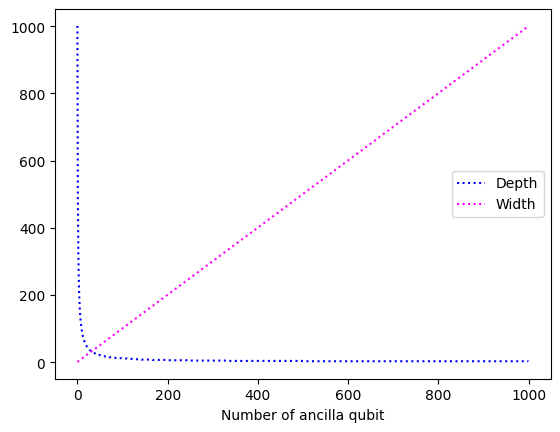
\includegraphics[scale=0.7]{plot.png}
        \caption{Depth and width scaling for the implementation of $R_{1000}$.}
        \label{fig:complexity}
    \end{figure}
    Write a function \verb|near_optimal_rz(n,psi,angles)| that returns the trade-off quantum circuit with the approximate optimal value $p^*$ of ancilla qubits.
    \item \textbf{Bonus}: It turns out that this method only works for diagonal unitaries. For an arbitrary unitary matrix of the form $\begin{pmatrix}
        \cos(\frac{\theta}{2}) & -e^{i\lambda}\sin(\frac{\theta}{2}) \\ e^{i\phi}\sin(\frac{\theta}{2}) & e^{i(\phi+\lambda)}\cos(\frac{\theta}{2})
    \end{pmatrix}$ one should find another method. Do you have any idea why?
\end{enumerate}
